\chapter{Úvod}

\section{Motivace projektu, záměr práce}
\label{introduction-motivation}

Při realizaci softwarových projektů zpravidla postupujeme od sběru požadavků, přes \emph{analýzu} a \emph{návrh} až k~\emph{fyzické realizaci} programového produktu ve zdrojovém kódu vhodného programovacího jazyka \cite{wiki:sdlc}. Vytvořením reprezentace systému ve zdrojovém kódu však životní cyklus softwarového díla nekončí. Vedle \emph{testování}, \emph{integrace}, \emph{akceptace} a \emph{dodávky} je nutné ještě uvažovat o~další fázi -- \emph{údržbě}. Pro tyto fáze, které jsou neméně důležité, leč mnohdy opomíjené, je kritická především \emph{architektura systému}.

Architektura existujícího systému je většinou definována poměrně vágně. Při dalších úpravách se tak můžeme spolehnout na malou podmnožinu pravidel, kterou u~daného systému předpokládáme a která často ani nemusí platit. Vždy se však můžeme spolehnout na to, že pokud zdrojový kód programového produktu projde bez chyb překladačem nebo interpreterem programovacího/skriptovacího jazyka, v~němž je napsán, jedná se o~kód podléhající pravidlům tohoto jazyka.

Syntaxe jazyka je definována gramatikou, sémantika potom dává jednotlivým konstruktům jazyka jejich význam (např. \verb+for+ bude znamenat opakované provádění kódu mezi počáteční \verb+{+ a koncovou \verb+}+ složenou závorkou následujícího bloku).

Kromě struktury, kterou vynucuje překladač jazyka bývá často zavedena množiná kódových konvencí. Vedle konvencí pro formátování zdrojového kódu (které nemají z~hlediska analýzy architektury systému význam) můžeme zmínit konvence, které zakazují aby měla metoda více než nějaký daný počet příkazů/parametrů, konvence, které nařizují, aby se v~kódu nevyskytovaly neprovolávané (mrtvé) části kódu, a další.

V~této práci se pokusíme zmíněné konvence zachytit jako pravidla, která lze vhodným způsobem ověřit. Znázornění tohoto konceptu je na obrázku \ref{work_scope}.
\begin{figure}[h!]
  \centering
  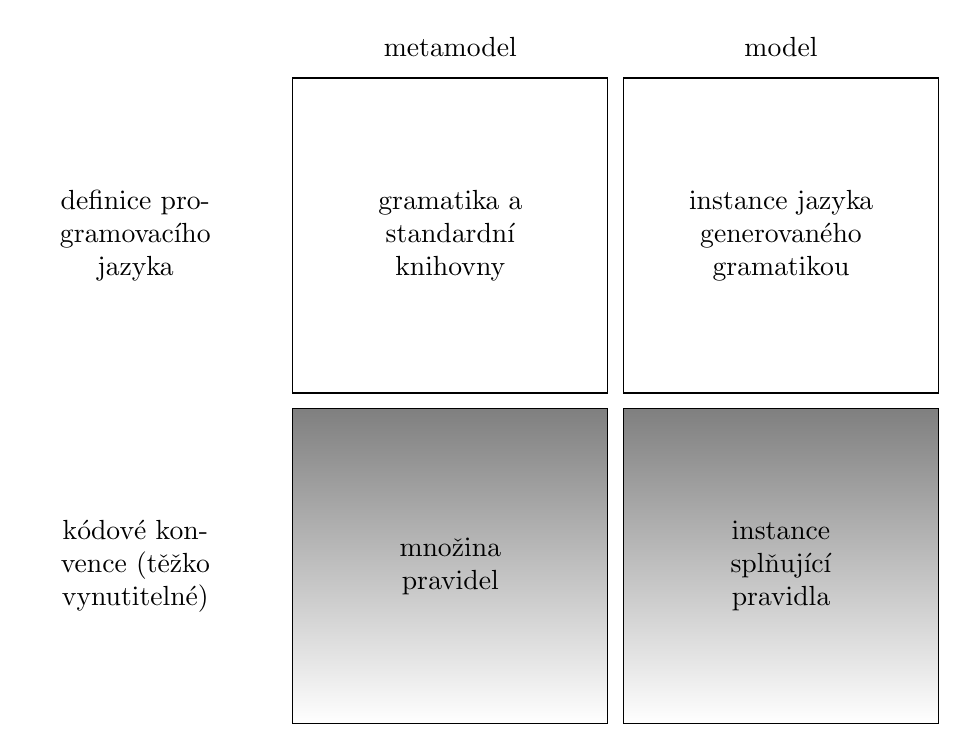
\begin{tikzpicture}
    \shadedraw  (0,0) rectangle (4,4);
    \shadedraw  (4.2,0) rectangle (8.2,4);
    \draw  (0,4.2) rectangle (4.0,8.2);
    \draw  (4.2,4.2) rectangle (8.2,8.2);

    \draw  (2,2) node[text width=2.5cm, text centered] {množina pravidel};
    \draw  (6.2,2) node[text width=2.5cm, text centered] {instance splňující pravidla};
    \draw  (2,6.2) node[text width=2.5cm, text centered] {gramatika a standardní knihovny};
    \draw  (6.2,6.2) node[text width=2.5cm, text centered] {instance jazyka generovaného gramatikou};

    \draw (-2,2) node[text width=2.5cm, text centered] {kódové konvence (těžko vynutitelné)};
    \draw (-2,6.2) node[text width=2.5cm, text centered] {definice programovacího jazyka};

    \draw (2,8.6) node[text width=2.5cm, text centered] {metamodel};
    \draw (6.2,8.6) node[text width=2.5cm, text centered] {model};
  \end{tikzpicture}
  \caption{Rozšíření gramatiky jazyka o~množinu pravidel.\label{work_scope}}
\end{figure}
Množina pravidel zpřesní metamodel tvořený gramatikou jazyka -- omezí množiny instancí daného jazyka na podmnožinu, která splňuje požadovaná pravidla.

Jistou analogii můžeme vidět ve značkovacím jazyku XML v~pojmech \emph{well-formedness} versus \emph{validita}. Gramatika udává, že se v~textu mohou vyskytovat elementy a atributy, že se nesmí \uv{křížit} jednotlivé tagy atd. Další dodatečná informace (DTD, XSchema, RELAX NG, atd.) potom zpřesní, jaké tagy, v~jakém pořadí a počtu se smí ve výsledné instanci XML dokumentu vyskytovat.

\section{Úvod do řešené problematiky}

Architektura softwarového systému \cite{wiki:software_architecture} je dána množinou pravidel a tvrzení o~uspořádání systému, která platí pro daný softwarový systém. Architekturu zpravidla uvažujeme z~různých pohledů (views) \cite{wiki:four_plus_one_views}, které popisují systémové komponenty a vztahy mezi nimi vždy z~úhlu některé ze zainteresovaných stran (stakeholders). Např. \emph{logical view} se zabývá architekturou z~pohledu funkcionality, kterou systém poskytuje \emph{koncovým uživatelům}, \emph{physical view} poskytuje pohled pro \emph{systémového inženýra} -- uspořádání komponent v~systému a propojení mezi nimi.

Pro systémového návrháře bude nejdůležitější právě architektura na fyzické úrovni, se kterou bude muset dále pracovat v~případě dodatečných zásahů do systému. Jedná se o~vztahy mezi konkrétními komponentami realizované v~existujícím systému. Ačkoliv sem spadají všechny komponenty systému (tedy i hardwarové), budeme se v~této práci zabývat zejména jeho softwarovými součástmi -- funkčními bloky a moduly.

Základní prostředky pro dělení softwarového díla na vhodné funkční moduly a bloky poskytuje již většina moderních programovacích jazyků. Různé programovací jazyky podporují různá paradigmata a následně i strukturování zdrojových kódů programu \cite{wiki:programming_paradigm}. Ve funkcionálním programovacím jazyku budeme strukturovat dílo do zanořených funkcí, u~objektově orientovaného programování budou základními moduly třídy a balíčky. V~textu práce se zaměříme právě na objektově orientované programovací jazyky.

Prostředky jazyka, které podporují správný návrh software rozšíříme navíc o~množinu pravidel tak, jak bylo uvedeno v~sekci \ref{introduction-motivation}. Množina těchto pravidel může být formulována neformálně ve formě požadavků na to, co by měla splňovat výsledná architektura. Uveďme příklady takových formulací:

\begin{itemize}
\item \uv{v~běžném kódu by se něměla vyskytovat (nestatická) pole s~modifikátorem \emph{public}, pouze \emph{private}, k~nimž se přistupuje pomocí \emph{getterů} a \emph{setterů}},
\item \uv{třídy z~balíčku A~nesmí záviset na jiných nesystémových \emph{třídách}, ale nejvýše na \emph{rozhraních} balíčku B} (programování proti rozhraní namísto proti konkrétní implementaci),
\item \uv{třídy v~tomto balíčku smí mít maximálně pět metod, z~nichž každá smí mít nejvýše tři parametry} (může být konvence v~nějaké firmě),
\item Law of Demeter.
\end{itemize}

Podobné neformální specifikace se pokusíme přeformulovat pomocí vhodně zvoleného formalismu do pravidel, která bude možné následně vyhodnotit a na základě výstupu buď navrhnout nebo (je-li to možné) opravit návrh tak, aby pravidla splňoval.

\section{Struktura práce}
% TODO: popis členění práce - co nalezne čtenář v jednotlivých kapitolách, jak je celé dílo strukturováno
% TODO: rozepsat přesně do odstavcového textu, přidat ref na jednotlivé kapitoly
% TODO: struktura práce by měla odpovídat fázím SDLC
\begin{itemize}
\item \emph{introduction} - úvod
\item \emph{requirements} - specifikace cílů práce
\item \emph{analysis} - analýza
\item \emph{design} - návrh
\item \emph{implementation} - implementace
\item \emph{testing} - testování
\item \emph{conclusion} - závěr
\item \emph{abbrev} - seznam použitých zkratek
\item \emph{diagrams} - uml diagramy % spise nebude, vse bude v textu prace
\item \emph{installation} - instalační příručka
\item \emph{used tools} - nástroje použité při realizaci práce
\item \emph{cdcontents} - obsah přiloženého CD
\end{itemize}
